\documentclass[11pt]{scrartcl}
\usepackage[secthm]{evan}
\usepackage{mathteam}

\author{Michael Luo}
\title{Dynamic Planet 2024-25 notes}
\date{\today}

\begin{document}

\maketitle

\begin{abstract}
	The 2024-25 Dynamic Planet binder for Science Olympiad. The topic is glaciers and my partner was Jos Buffington.

	We first begin with some of my personal notes, then include two practice tests. We also include Chapter 18 of Lutbuck.
\end{abstract}

\begin{figure}[H]
	\centering
	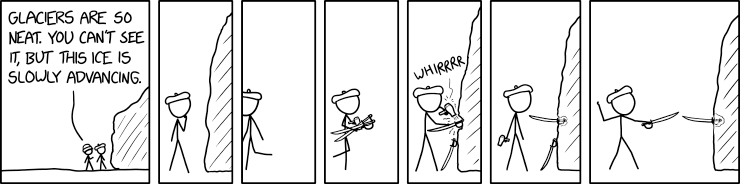
\includegraphics[width=1\textwidth]{glacier.png}
	\caption{The Norwegian adaptation of The Sword in the Stone takes things in a weird direction. Source: \url{www.xkcd.com/2164}.}
\end{figure}

\tableofcontents

\pagebreak

\section{Notes from Lutbuck chapter 18}\label{sec:lutbuck}

\epigraph{TO-GO is short for TOO GOOD}{the Culver's frozen custard refrigerator}

\subsection{General definitions on glaciers}

I think the main point from this section is that glaciers and rivers are basically the same, except glaciers are slower and they carry way more stuff. I believe the relevant term is \emph{competence}.

\begin{itemize}
	\ii A \emph{valley glacier} is one in a valley. Duh. They are also called \emph{alpine glaciers}.
	\ii An \emph{ice sheet} is a big glacier covering a large area of land. Examples: Greenland and Antarctica.
	\ii The \emph{Last Glacial Maximum} is exactly what it sounds like. There have been many glacial and interglacial periods throughout the Quaternary period, this is the last one.
	\ii An \emph{ice shelf} is formed when an ice sheet flows into the ocean. We say an ice shelf is \emph{grounded} if it touches bottom. As an ice shelf melts, it drops stones called \emph{dropstones} (great name), which is evidence for the existence of glaciers.
	\ii An \emph{ice cap} is an ice sheet but smaller. Example: Vatnaj\"okull ice cap in Iceland.\footnote{Did you know that the Vatnaj\"okull ice cap is predicted to melt within the next $50$ years? No cap.}
	\ii An \emph{outlet glacier} is a glacier produced by an ice cap or sheet. They produce icebergs when they reach the sea.
	\ii A \emph{piedmont glacier} is a valley glacier that escaped the valley and spread out like a puddle.
	\ii \emph{Firn} is the really gross snow that's dense, shitty, dirty, and basically a bunch of ice crystals. This is produced by pressure from snow above. Once there are around $50$ meters of snow, firn becomes ice.
	\ii \emph{Plastic flow} happens when ice flows, starts below $50$ meters.
	\ii \emph{Basal slip} is sliding from ice in contact with the bedrock.
	\ii The \emph{zone of fracture} is above $50$ meters. It's when ice fractures. Produces crevasses, depth of those is restricted to $50$ meters.
	\ii The \emph{zone of accumulation} is the area where more snow falls each winter than melts in the summer. The \emph{zone of wastage/accumulation} is the opposite, the line dividing the two is called the \emph{snowline/equilibrium line}. The \emph{glacial budget} is whether a glacier is retreating, advancing, or at equilibrium.
	\ii Glaicers erode by \emph{plucking} and \emph{abrasion}. Plucking occurs when meltwater pulls rock loose by freezing under a rock. Abrasion occurs when stone is scratched by plucked stones; this produces \emph{rock flour} (which is unfortunately not edible). \emph{Glacial striations} are large scratches produced in bedrock by huge ice fragments' abrasion, they are linear and help one to reconstruct the direction of glacial flow.
\end{itemize}

\subsection{Erosional features}

It begins.

\begin{itemize}
	\ii An \emph{glacial trough} or a \emph{glaciated valley} is a U-shaped valley. 
	\ii A \emph{hanging valley} is a cliff formed by the height difference from erosion from a main and a tributary glacier. A \emph{truncated spur} is a cliff formed when a mountain is orthogonal to a glacial trough.
	\ii A \emph{pater noster lake} is a depression formed by plucking filled with water.
	\ii A \emph{cirque} is a three-sided bowl-shaped depression at the origin of the glacier.
	\ii A \emph{tarn} is a lake in a cirque.
	\ii A \emph{col} is a pass formed when two cirques meet. A \emph{ar\^ete} is a ridge formed when two cirques meet. A \emph{horn} is a peak formed when three cirques meet. Example: the Matterhorn.
	\ii A \emph{roche moutonn\'ee} is an erosional feature formed when an existing slope is smoothed by glacier movement. The less steep side is ``upstream.''
	\ii A \emph{fiord} is a glacial trough flooded by seawater, either due to sea-level rise or because glaciers eroded below sea level.
\end{itemize}

\begin{figure}[H]
	\centering
	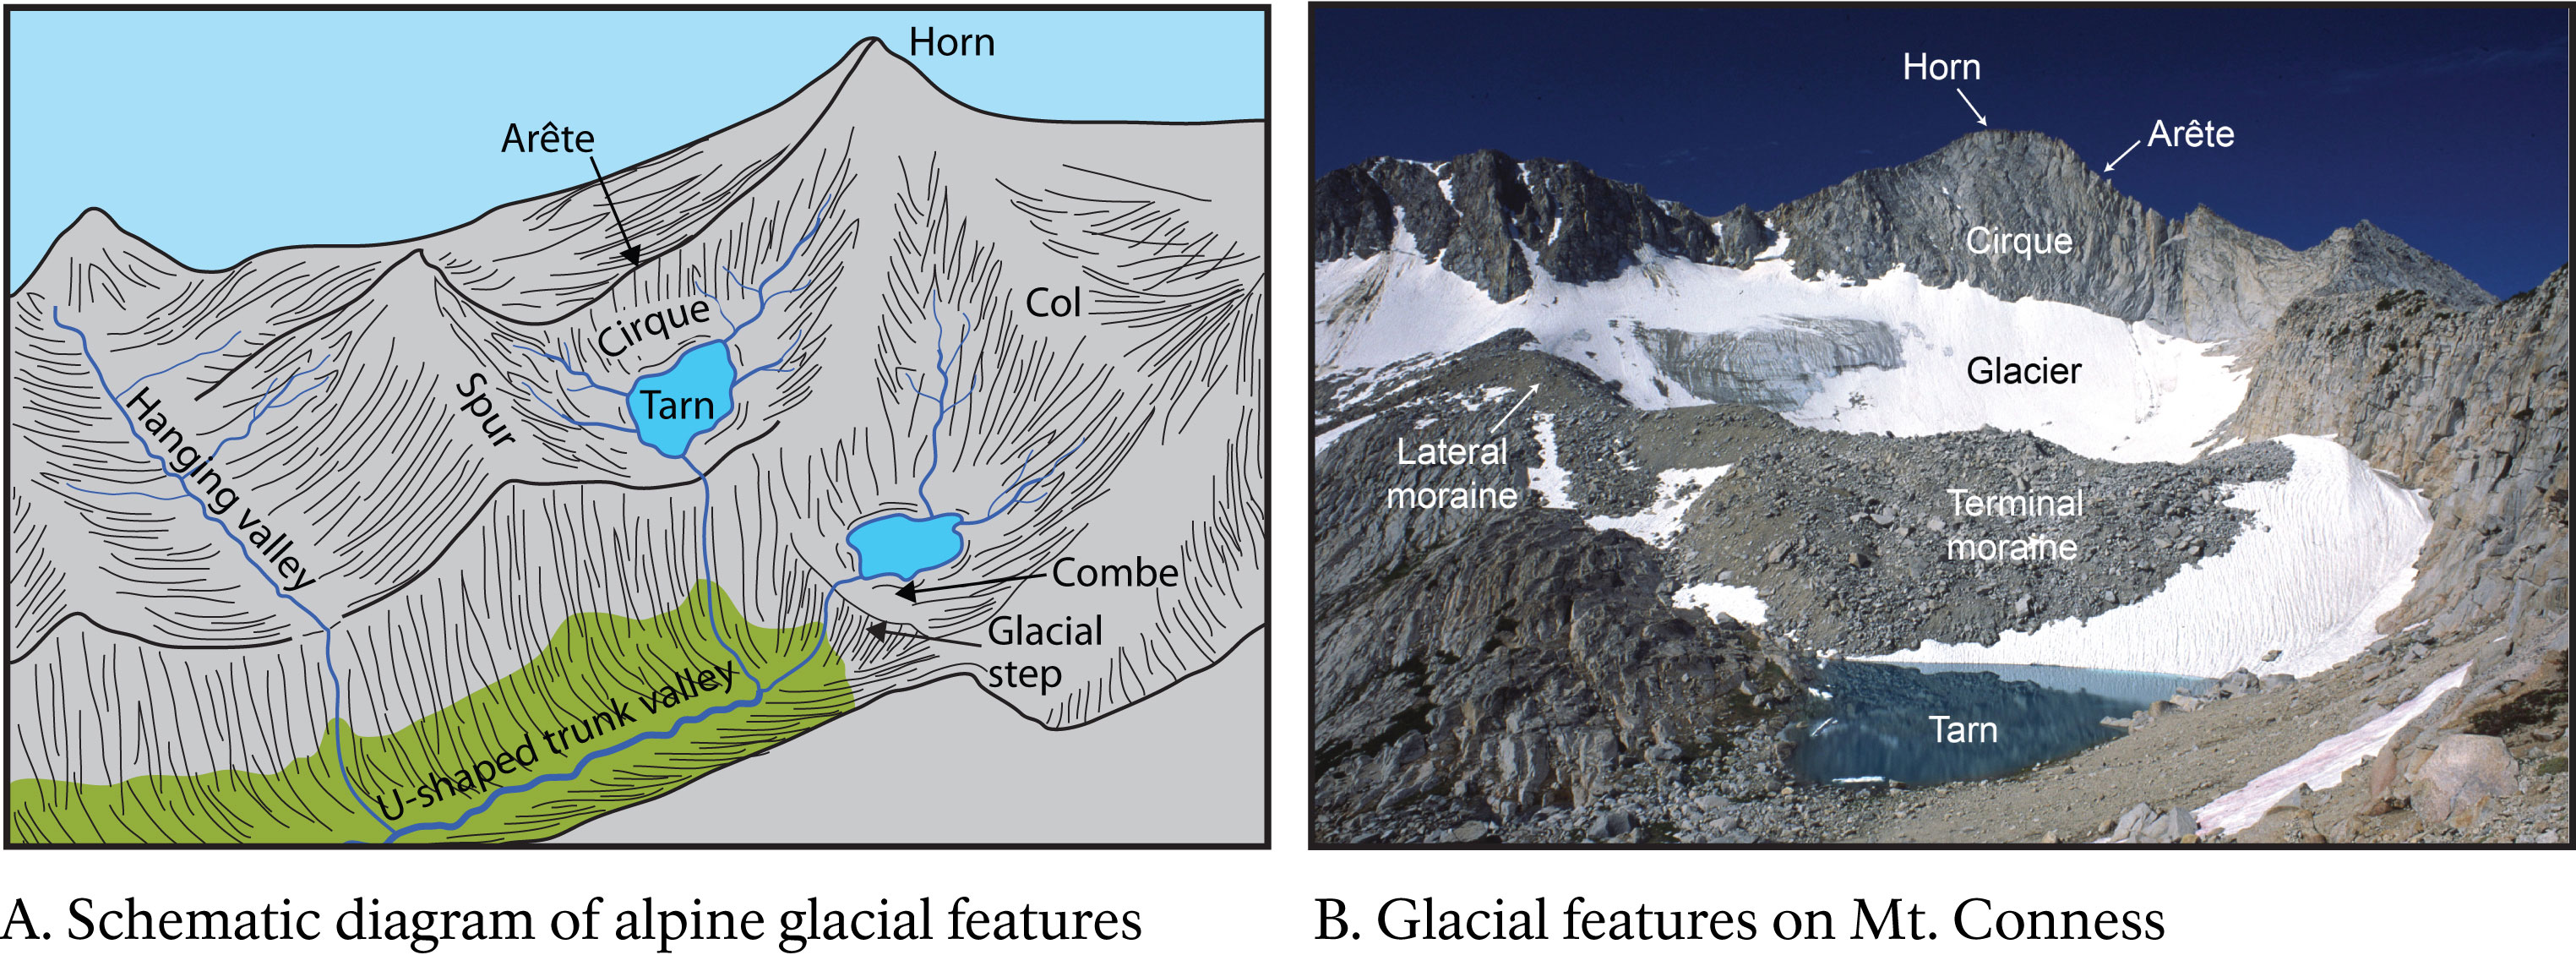
\includegraphics[width=1\textwidth]{big_erosion.jpg}
	\caption{Some alpine glacial features. Source: \url{https://commons.wikimedia.org/wiki/File:YOSE_29_Glacial-features_WEB.jpg}}
\end{figure}

\subsection{Depositional features}

\begin{itemize}
	\ii \emph{Glacial drift} is sediment deposited by glaciers. \emph{Till} is directly dropped by the glacier; \emph{stratified drift} is from glacial meltwater. In particular, till is unsorted while stratified drift is sorted.
	\ii A \emph{glacial erratic} is a boulder different from the bedrock below transported by glaciers.
\end{itemize}

\subsubsection{Landforms made of till}

\begin{itemize}
	\ii A \emph{moraine} is a layer of till. A \emph{lateral moraine} is from the residue on the sides of the valley, a \emph{medial moraine} is formed when two glaciers (and their lateral moraines) meet.
	\ii An \emph{end moraine} is a layer of till formed at the terminus of a glacier. A glacier is essentially a conveyor belt---the sediment all gets dropped to the end. Multiple can form, the one ``furthest along'' is called the \emph{terminal end moraine}; the other ones are called \emph{recessional end moraines}. Long Island is an end moraine.
	\ii A \emph{ground moraine} is a flat-ish layer of till deposited as a glacier retreats.
	\ii A \emph{drumlin} is a hill formed by till. Don't confuse it with a roche moutonn\'ee: this is depositional and the steep side is ``upstream.'' Example: Bunker Hill (!!). They are found in drumlin fields.
\end{itemize}

\subsubsection{Landforms made of stratified drift}

There are two general types: \emph{ice-contact}, which are formed in contact with ice. Obviously. And there is outwash, which is deposited away from the glacier by meltwater streams.

Here are the outwash ones:

\begin{itemize}
	\ii An \emph{outwash plain} (ice sheet) or a \emph{valley train} (valley glacier) is a ramp-like feature just outside an end moraine formed by sand of gravel that is deposited quickly as meltwater slows.
	\ii A \emph{kettle} is a depression formed by the following process: a persistent piece of glacial ice exists, the remaining area is covered with sediment, the ice melts. Example: Walden Pond (!!).
\end{itemize}

Here are the ice-contact ones. Ice-contact deposits form on top of a glacier, then gets dropped when the glacier melts.
\begin{itemize}
	\ii A \emph{kame} is a mount or steep-sided hill, formed by deposited sediment in a delta, fan, or an opening in the ice.
	\ii A \emph{kame terrace} is a narrow, linear feature formed on the side of a valley. Basically the same as a kame.
	\ii An \emph{esker} is a very long, narrow, sinuous ridge formed by dropped sand and gravel.
\end{itemize}

\begin{figure}[H]
	\centering
	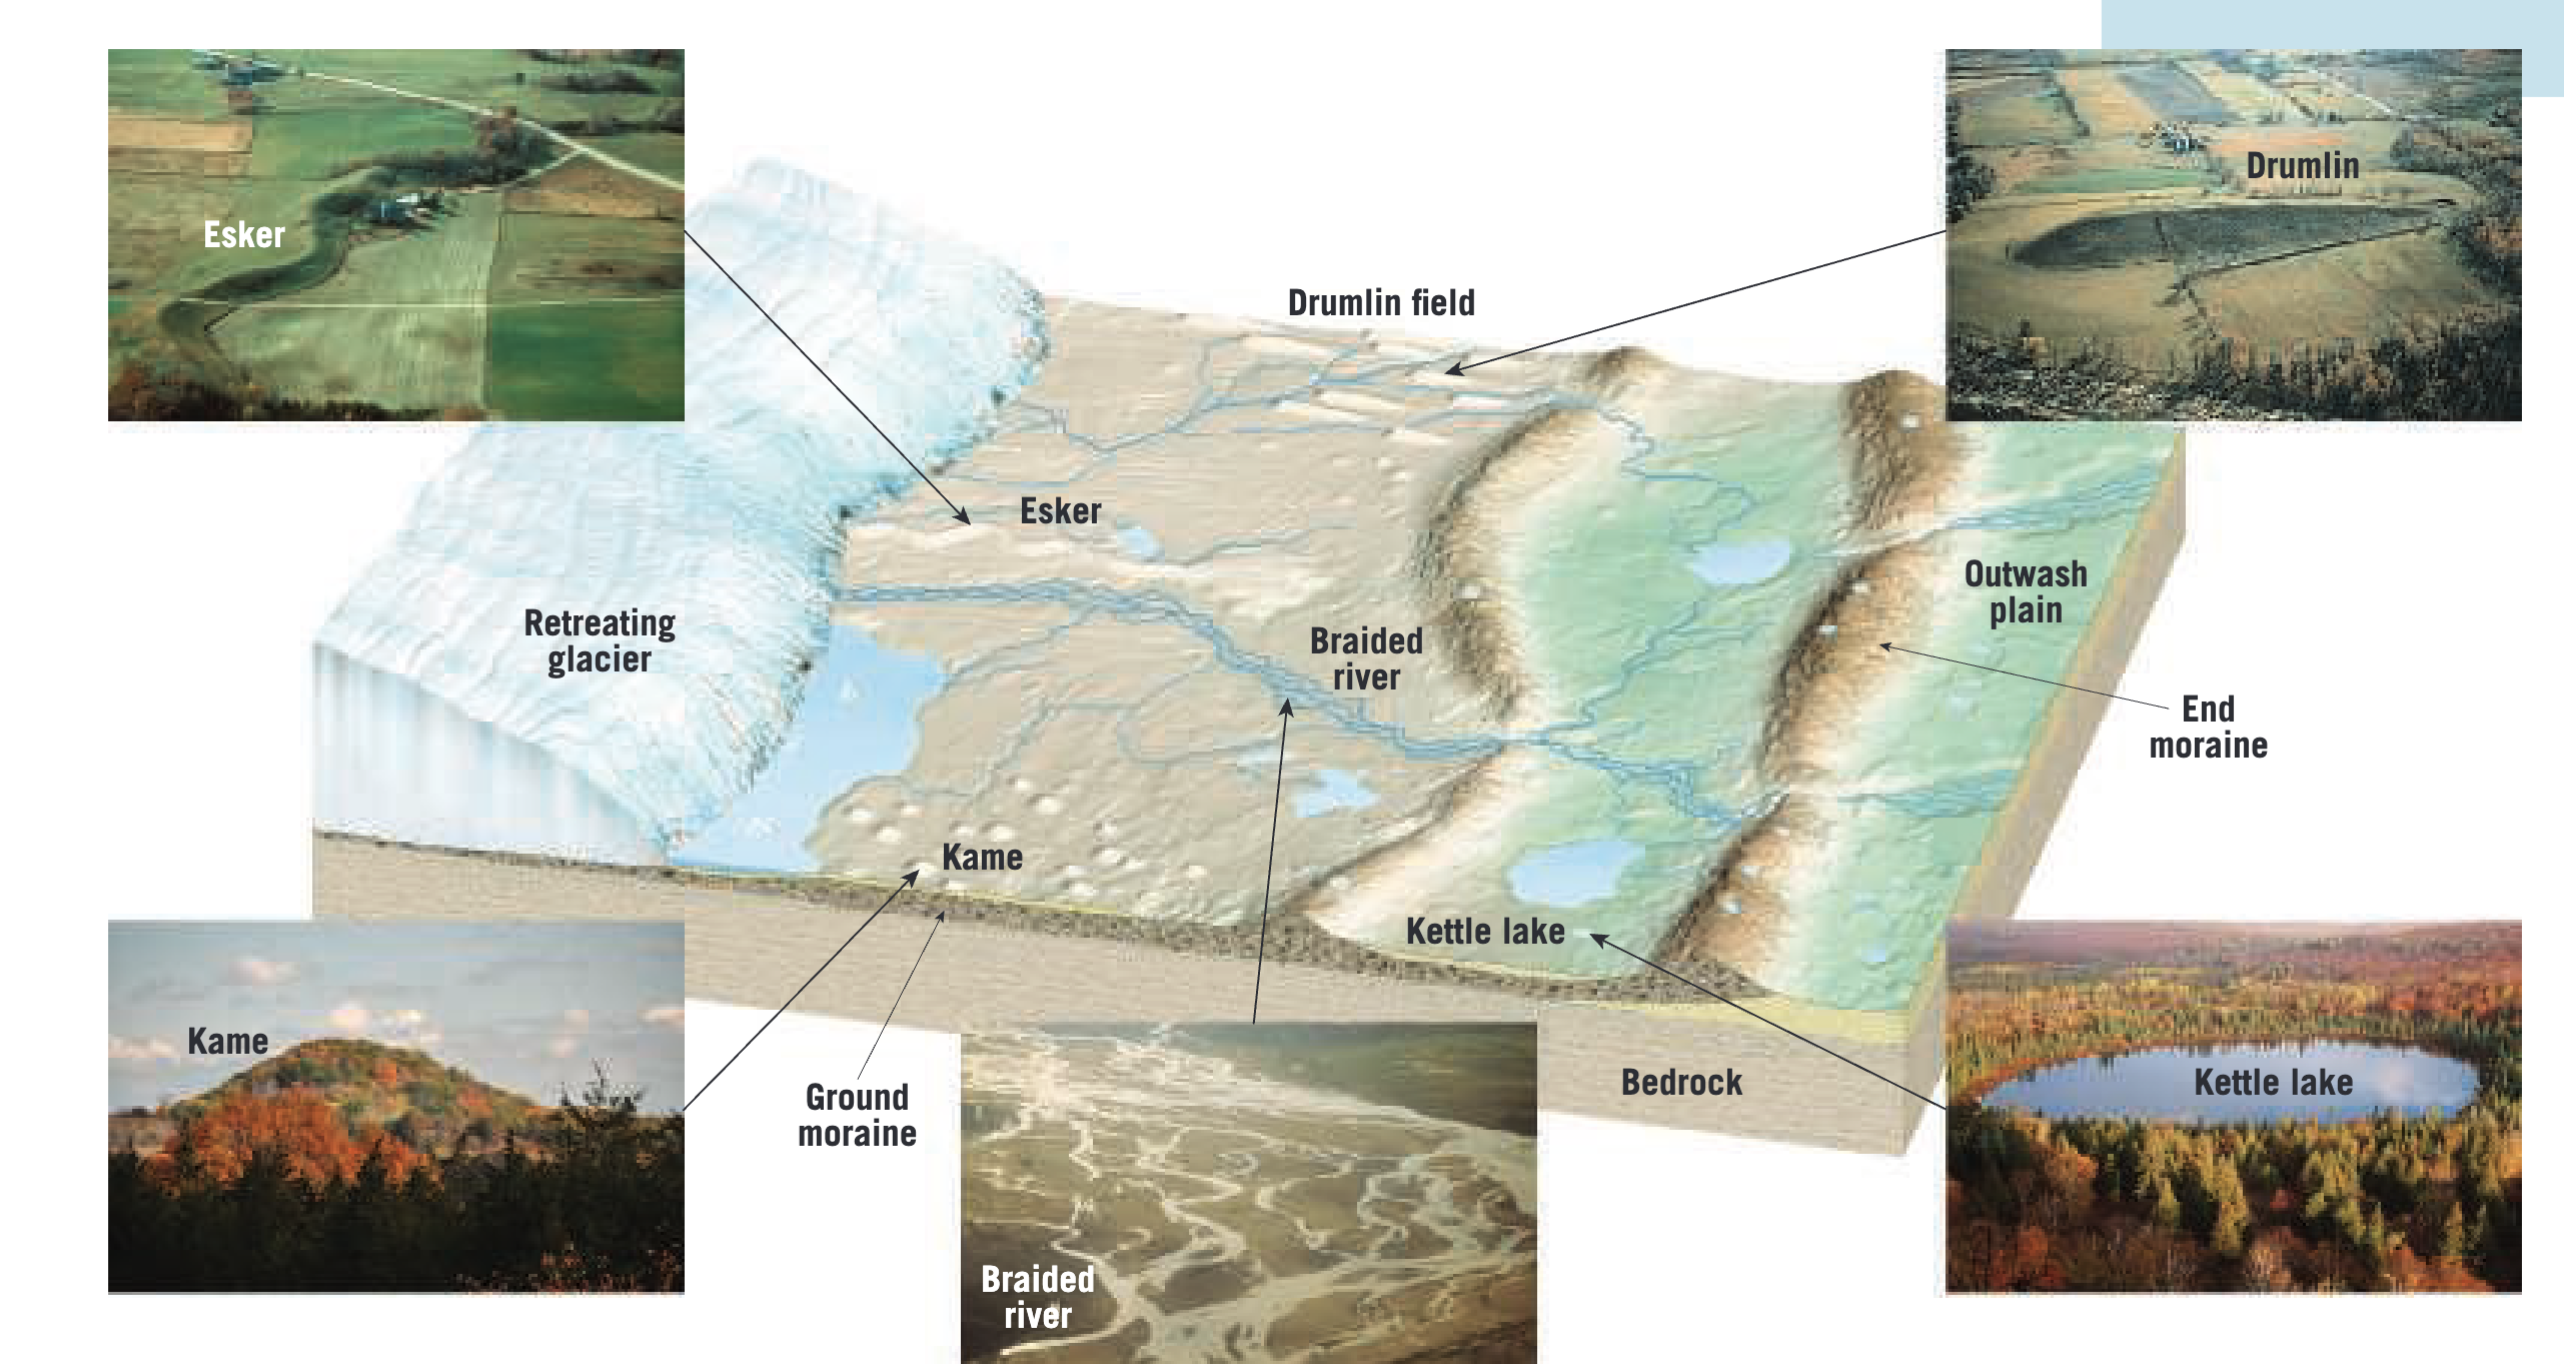
\includegraphics[width=1\textwidth]{retreat.png}
	\caption{A retreating glacier with some common features.}
\end{figure}

\subsection{Miscellanous}

\begin{itemize}
	\ii Your mother (very heavy) stands on a trampoline, and it sinks. When she leaves, the trampoline slowly returns turns to its original position. This is \emph{isostatic rebound}, but your mother is an ice-age glacier and the trampoline is the Earth's crust. It's still rebounding from the Last Glacial Maximum.
	\ii Glaciation changes rivers and the hydrological landscape in general---the Great Lakes were produced by glacier erosion.
	\ii \emph{Lake Agassiz} was a lake bigger than all the Great Lakes combined. Agassiz is an example of a \emph{proglacial lake}, a lake just outside a glacier or an ice sheet formed by glacial meltwater.
	\ii The colder climate in ice ages produces \emph{pluvial lakes}, which are fed by rain. (The colder climate reduces evaporation.) Lake Boneville was a pluvial lake comparable to Lake Michigan. The Great Salt Lake is its residue.
	\ii Glacial cycles and ice ages are controlled by the Milankovitch cycles, which are eccentricity, obliquity, and precession.
\end{itemize}

\begin{figure}[H]
	\centering
	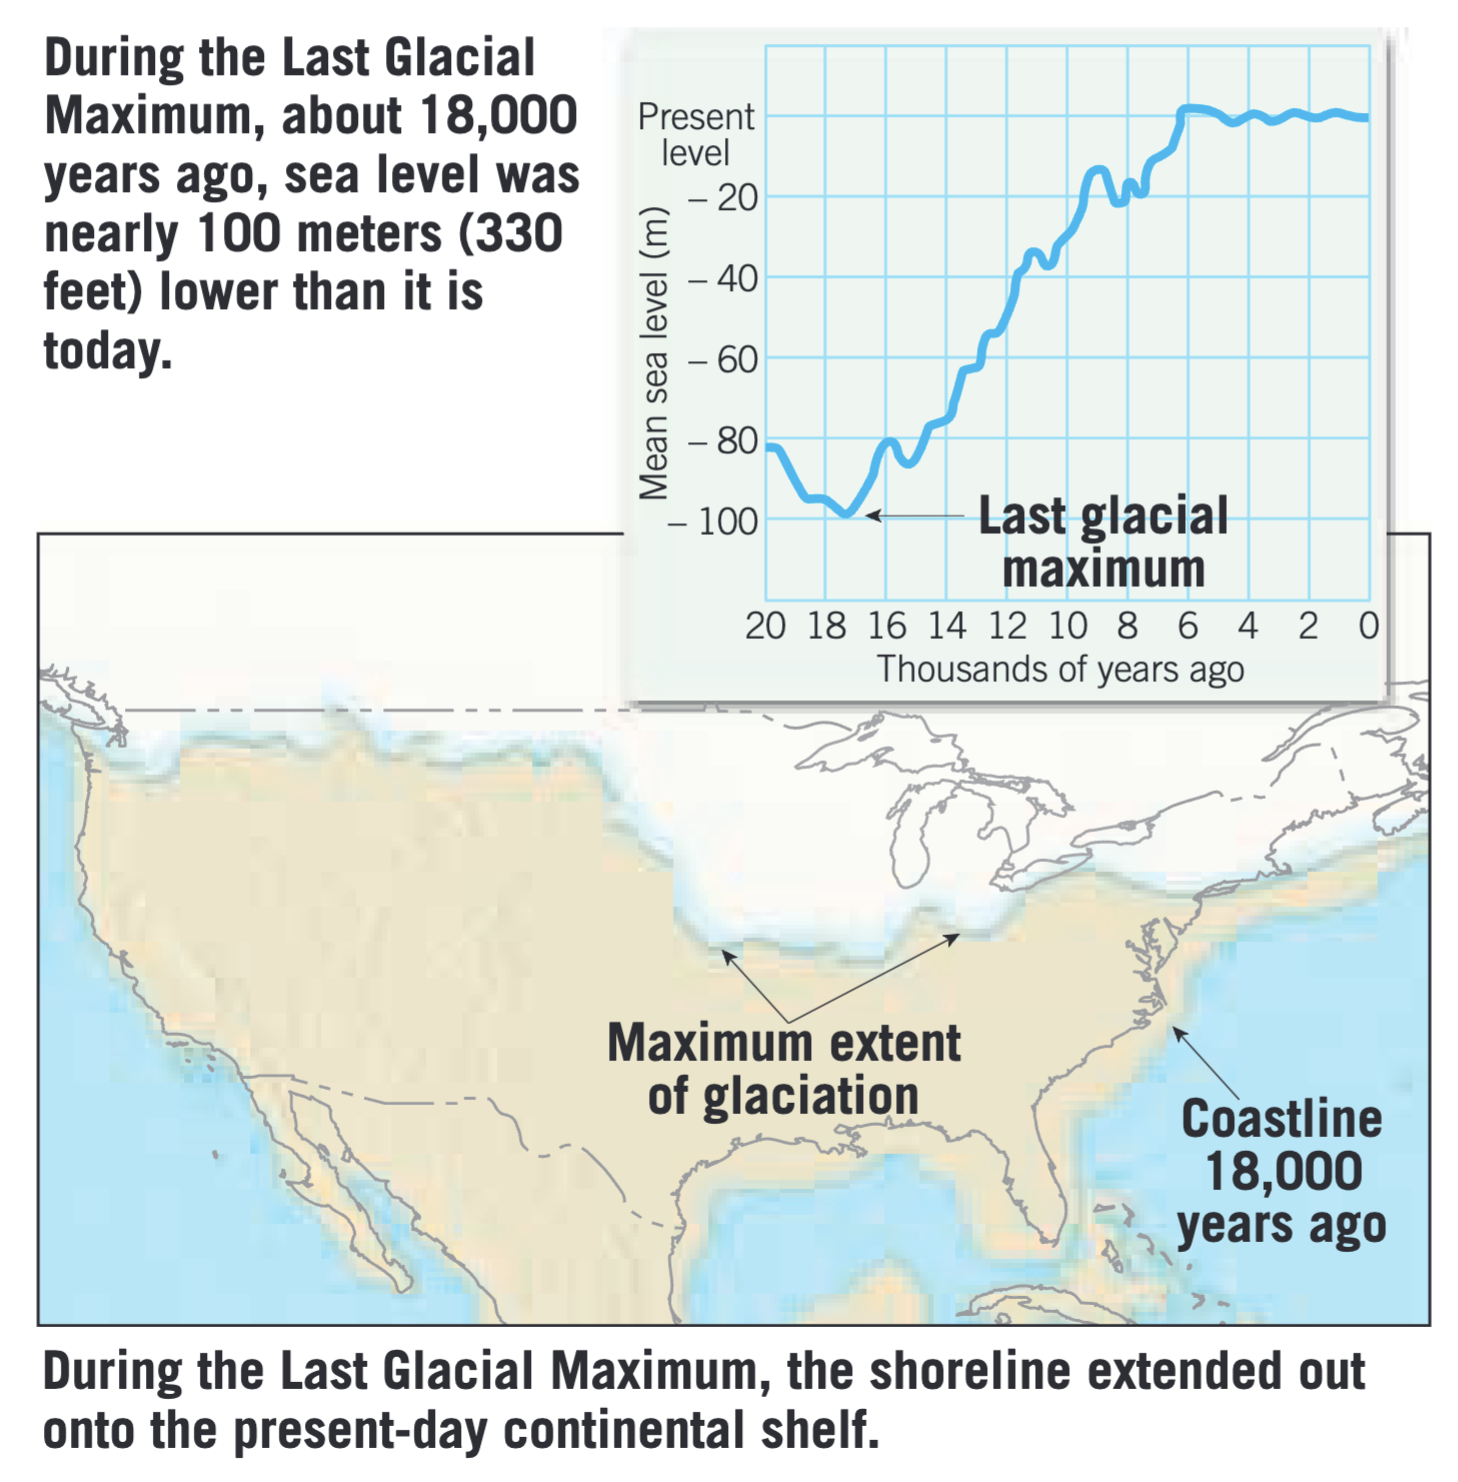
\includegraphics[width=0.5\textwidth]{last_glacial_maximum.png}
	\caption{A world I really do not want to live in.}
\end{figure}

\section{Literally every item on the rules}

\epigraph{I don't know no nothin' `bout no ice, I'm just cold}{KSI in ``Thick of It''}

Lots of repeats with the above. Space is not a problem for me though, since I have a million-dollar ink budget.

\begin{itemize}
	\ii \textbf{Glacier formation.} The crystal structure of ice is shown in \Cref{fig:ice_crystal}. N\'ev\'e is relatively new snow which melts a little, refreezes a little, and gets compacted a little. Once it survives for a year, it becomes firn. After firn gets buried by $50$ meters of snow, it becomes glacial ice. The zones of ablation and accumulation is where a glacier is net gaining/losing ice, respectively; the equilibrium line seperates them. Basal sliding is when the entire glacier slides along the bottom, plastic flow is like a very viscous liquid flowing.
	\begin{figure}[H]
		\centering
		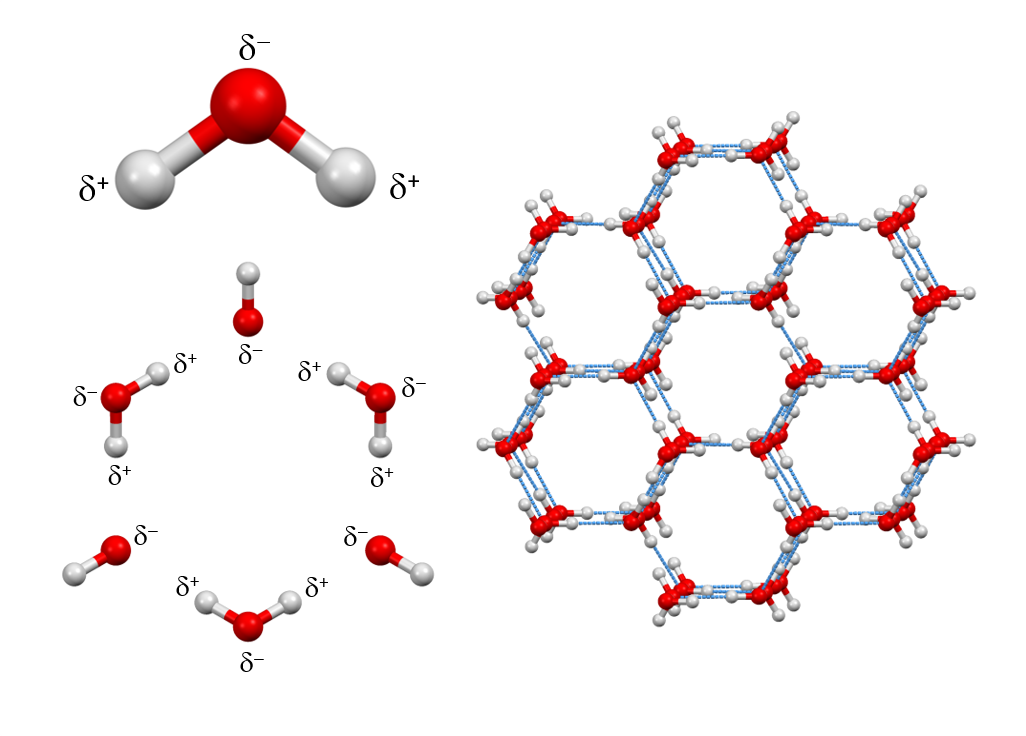
\includegraphics[width=0.5\textwidth]{ice_crystal.png}
		\caption{The crystal structure of ``normal'' hexagonal ice.}
		\label{fig:ice_crystal}
	\end{figure}	
	\ii \textbf{Types of glaciers and their geographic distributions.} Valley/alpine glaciers are found in (you guessed it) valleys, where the upstream endpoint is a cirque. A hanging glacier is one that stops at a cliff. A piedmont glacier is an alpine glacier that reached the end of its valley and spilled out.
	
	An ice sheet is a\dots{} sheet of ice, like Greenland or Antarctica. An ice stream is a fast-moving ``river'' within an ice sheet. An ice shelf is part of an ice sheet that spilled out into the ocean, usually generated by ice streams. An ice rise is an ice hill on an ice sheet. An ice cap is a small ice sheet, like the Vatnaj\"okull ice cap in Iceland. An ice tongue is a floating ice shelf.
	\ii \textbf{Features in glacial ice.} A crevass is a crack in the ice above $50$ meters, created by internal forces to the ice. An icefall is an area of a glacier that is steep and moves much faster than the surrounding areas, like an ice stream but steeper and within alpine glaciers.
	
	Ogives are wavelike features formed below icefalls with each wave corresponding to one year of ice flow. Ice speed is far greater in an icefall than average, so it stretches out. So ice is thinner on an icefall, so in summer as icefalls melt, much more melts compared to other spots on the glacier. More melting reveals more debris and dust inside the ice, creating the dark bands. Ice that spends winter in the icefall is able to accumulate more snow and reveal less debris, emerging from the icefall as the light bands. Glaciers flow faster in the middle, so the bands become arcs.\footnote{The preceding section about ogives was blatantly plagiarized from \url{https://juneauicefield.org/blog/2015/8/8/ogives-glacial-masterpieces}.}
	
	Calving is when icebergs break off from a glacier. The marine ice sheet instability hypothesis is as follows: as some of Antarctica melts, the grounding line will move inland, then since the west Antarctic ice sheet has a reverse gradient, this will destabilize West Antarctica and speed up melting. Ice shelf buttressing means that ice sheets support and stabilize each other; so if some of Antarctica melts, we are all cooked.
	\ii \textbf{Formation of landscape features by glaciers.} Cirques, U-shaped valleys, ar\^etes, horns, striations, r\^oche moutonn\^ees, moraines, kames, drumlins, eskers, erratics, tarns, kettles, and proglacial lakes are covered in \Cref{sec:lutbuck}. A \emph{tor} is a freestanding naturally occuring rock stack formed by erosion. Everyone knows what the Great Lakes are, the Finger Lakes are a set of $11$ lakes in New York formed by moraines, and moraine-dammed lakes are exactly what they sound like.
	\ii \textbf{Periglacial processes and landforms.} Permafrost is ground that is frozen for at least two years. On top of permafrost, there is a very thin active layer that thaws in the summer. A pingo is a hill filled with permafrost; their formation is shown in \Cref{fig:pingo}.
	\begin{figure}[H]
		\centering
		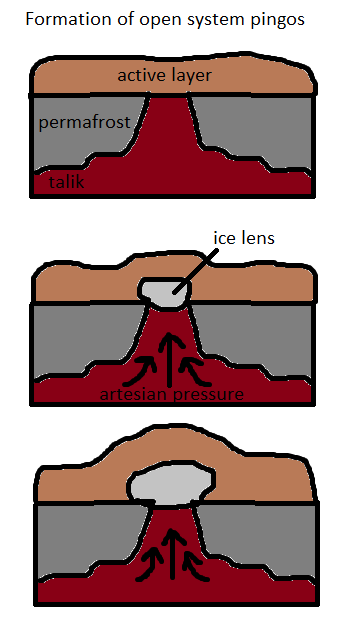
\includegraphics[width=0.3\textwidth]{hydraulic_pingo.png}
		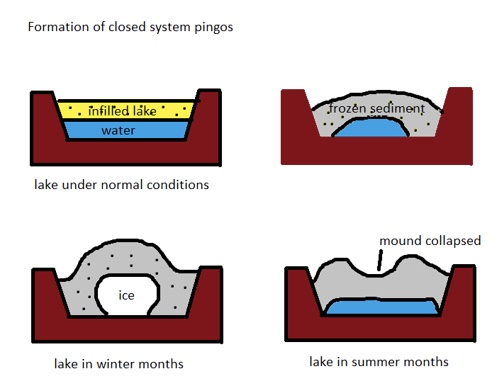
\includegraphics[width=0.6\textwidth]{hydrostatic_pingo.jpg}
		\caption{Formation of open (left) and closed (right) system pingos. An \emph{talik} is an area of unfrozen ground covered by permafrost.}
		\label{fig:pingo}
	\end{figure}
	\ii \textbf{Sea ice.} An ice floe is a large pack of floating ice at least $20$ meters wide.\footnote{From Wikipedia.} Freeboard thickness is from the top of the ice to the water level. Draft thickness is from sea level to the bottom. A pressure ridge is formed when two ice floes collide, as shown in \Cref{fig:pressure_ridge}. Frazil ice is a collection of tiny ice crystals formed by supercooled water, pancake ice is formed by colliding frazil ice or slush. Fast ice is ironically ice that does not move---it is ``fastened'' to land. Newer ice tends to be closer to land, older ice tends to get pushed away.

	A \emph{lead} is a temporary linear crack in sea ice that typically refreezes quickly that could connect to the open ocean. A \emph{polynya} is a more circular opening in sea ice, typically surrounded by ice. Polynyas are formed by two main processes:
	\begin{itemize}
		\ii A \emph{sensible heat polynya} occurs when warm water upwelling keeps the surface water temperature at or above the freezing point. This reduces ice production.
		\ii A \emph{latent heat polynya} is formed by winds continually blowing newly-formed ice away from a fixed point. Latent heat polynyas contribute to the formation of sea ice production.\footnote{From Wikipedia.}
	\end{itemize}
	Leads and polynyas allow land animals to feed and allow aquatic mammals to breathe.
	\ii \textbf{Glacial hydrology.} Surface melt and lakes are exactly what they sound like. A moulin is a nearly-vertical ``river'' from the top of the glacier to the bottom. The meltwater lubricates the bottom and helps with basal slip. A subglacial lake is a lake under a glacier.
	\begin{figure}[H]
		\centering
		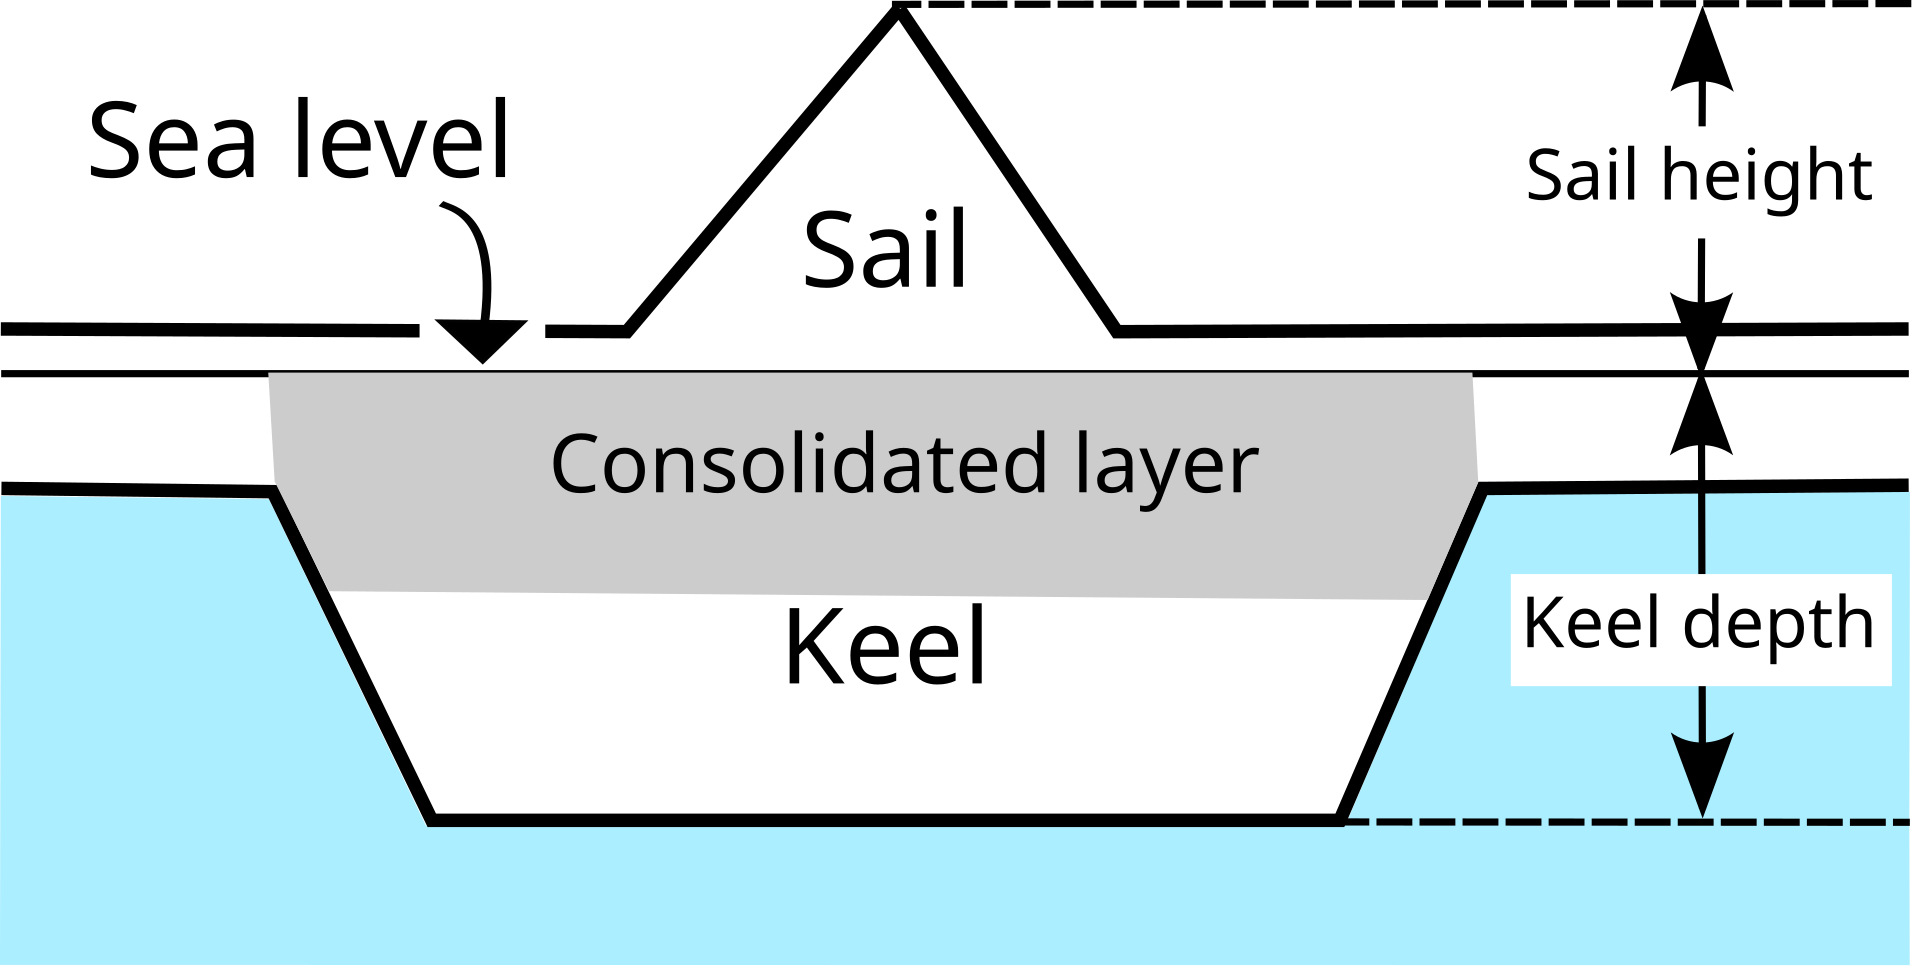
\includegraphics[width=0.5\textwidth]{pressure_ridge.png}
		\caption{An idealized pressure ridge.}
		\label{fig:pressure_ridge}
	\end{figure}
	\ii \textbf{Global connections of glaciation.} Glacial cycles are controlled by the Milankovitch cycles, which are eccentricity, obliquity, and precession.
	\ii \textbf{History of ice on Earth and its evidence.} I hate this event. Why can't I just do Fermi. Evidence for glaciation includes drop stones, erratics, striations, etc. Snowball Earth is a theory that the Earth was basically totally frozen (including the oceans). The Eocene-Oligocene extinction event was caused by glaciation and rapid temperature drops. After the Drake Passage was opened, we were saved from glaciers since Antarctica was cut off by the Antarctic Circumpolar Current. The Laurentide Ice Sheet produced Lake Agassiz. More recently, basically everything has been retreating as the result of human climate change.
	\ii \textbf{Sedimentary sequences produced in glacial environments.} A varve is an annual layer of sediment or sedimentary rock, formed by glacier melt/freeze cycles.
	\ii \textbf{Methods of studying glaciers and interpretation of related data.} All the standard survey techniques, plus gravimetry, which is measuring the strength of a graviational field (!!). Ice cores can be used for radiometric dating, analysis of the amount of snow each year (colors give summer/winter cycles), temperature history (oxygen isotope analysis), relative humidity, wind speed (from deuterium isotope analysis), history of cosmic rays (from beryllium-10), and paleoatmospheric analysis.

	In particular, more oxygen-18 in seawater implies the world is colder.
	\ii \textbf{Glacial hazards, including but not limited to ice avalanches and glacial lake outburst floods.} I think we all know what these are.
\end{itemize}

\section{Numerical facts}

\epigraph{Chilling like a villain}{}

A section entirely consisting of numerical facts for quick lookup.

\subsection{Height, thickness, area}

\begin{itemize}
	\ii Antarctic sea ice is around $1$ to $2$ meters thick, while Arctic sea ice is usually $2$ to $3$ meters thick.
	\ii Antarctic glacial ice is on average $2.16$ kilometers thick.\footnote{From \url{https://www.antarctica.gov.au/about-antarctica/ice-and-atmosphere/ice-sheet/}.}
	\ii Valley glaciers usually have an average thickness of less than $100$ meters, but they can be more than $300$ meters thick, like Catherine Xu horizontally.
	\ii Ice sheets currently cover around $10$ percent of Earth's land area. Ice sheets covered around $8$ percent of the Earth and $25$ percent of its land area during the Last Glacial Maximum.
	\ii During the Last Glacial Maximum, the sea level was around $100$ meters lower than today. If Antarctica melted, sea level would be $60$ to $70$ meters higher.
\end{itemize}

\subsection{Dates}

\begin{itemize}
	\ii The Milankovitch cycles eccentricity, obliquity (degree of tilt), and precession (direction of tilt) have periods of $100000$ years, $41000$ years, and $26000$ years, respectively.\footnote{From \url{https://science.nasa.gov/science-research/earth-science/milankovitch-orbital-cycles-and-their-role-in-earths-climate/}.}
	\ii Snowball Earth (if it occured) most likely occured $550$ to $725$ million years ago during the Neoproterozic.
	\ii The Eocene-Oligocene extinction event occured $34$ million years ago.
	\ii The Quaternary period began $2.6$ million years ago.
	\ii The Laurentide Ice Sheet existed from the beginning of the Quaternary to the Last Glacial Maximum.
	\ii The Last Glacial Maximum was from $26000$ to $20000$ years ago.
	\ii Lake Agassiz existed from $12000$ to $7500$ years ago.
\end{itemize}

\subsection{Miscellanous}

\begin{itemize}
	\ii Glacial erratics can be transported up to $600$ miles.
	\ii Drumlins are around $15$ to $50$ feet high and a kilometer long.
	\ii Kettle lakes are at most $2$ kilometers in size, but in Minnesota they can be up to $10$.
	\ii Ice has density $0.91$ times that of water.
	\ii Glacial flow rates range from $2$ to $800$ meters per year. Some glaciers surge.
	\ii Earth's average albedo is around $0.3$.
\end{itemize}

\begin{comment}

\section{Notes from the Boyceville exam}

\begin{itemize}
	\ii Australia is the only continent without glaciers, due to its low latitude, low elevation, its dryness.
	\ii Lake color is affected by sediment and depth. The deeper/less sediment, the bluer.
	\ii A bog is spongy ground.
	\ii Kettle lakes disappear when permafrost melts, allowing the ground to become permeable.
	\ii The headwall of a glacier is the rocky wall at the top of the glacier.
	\ii The toe, terminus, or snout of a glacier is its lowest point.
	\ii The most recent glacial period was called the Wisconsinan Glaciation.
	\ii Albedo is the fraction of light a surface reflects. A pure white object has albedo $1$. Earth's average albedo is around $0.3$.
\end{itemize}

\end{comment}

\end{document}